\documentclass[11pt,a4paper]{article}
\usepackage[utf8]{inputenc}
\usepackage[T1]{fontenc}
\usepackage{graphicx}
\usepackage{amsmath}  % Math support
\usepackage{amsfonts} % Extra math symbols
\usepackage{booktabs} % For tables
\usepackage{array}    % Table formatting
\usepackage{enumitem} % Compact lists
\usepackage{fancyhdr} % For custom header
\usepackage[backend=biber,style=authoryear]{biblatex}  % For citations and bibliography
\usepackage{amssymb} % For independence symbol
\usepackage{hyperref} % For linking footnotes

% Minimalistic header
\pagestyle{fancy}
\fancyhf{} % Clear default header and footer
\fancyhead[L]{\small Juliet Fleischer \hfill Januar 2025}  % Left-aligned header with name and date

% Margins and layout adjustments
\setlength{\hoffset}{-18pt}
\setlength{\oddsidemargin}{0pt} 
\setlength{\evensidemargin}{0pt}
\setlength{\marginparwidth}{54pt}
\setlength{\textwidth}{481pt}
\setlength{\voffset}{-18pt}
\setlength{\marginparsep}{7pt}
\setlength{\topmargin}{0pt}
\setlength{\headheight}{12pt}  % Minimal height for the header
\setlength{\headwidth}{490pt}
\setlength{\headsep}{10pt}  % Space between header and text
\setlength{\footskip}{27pt}
\setlength{\textheight}{720pt}

% Bibliography file
\addbibresource{../literature.bib}  % Your exported .bib file


\begin{document}

\section{Fairness Metrics \parencite{verma2018}}

\subsection*{Independence $\hat{Y} \perp A$}
\begin{itemize}[leftmargin=2em]
    \item Statistical Parity/Demographic Parity: $P(\hat{Y} = 1 \mid A = a) = P(\hat{Y} = 1 \mid A = b)$
    \item Conditional Statistical Parity: $P(\hat{Y} = 1 \mid E = e, A = a) = P(\hat{Y} = 1 \mid E = e, A = b)$ \\ \textit{E is a set of legitimate features that may affect the outcome.}
\end{itemize}

\subsection*{Separation $\hat{Y} \perp A \mid Y$}
\begin{itemize}[leftmargin=2em]
    \item Equalized Odds: $P(\hat{Y} = 1 | Y = y, A = a) = P(\hat{Y} = 1 | Y = y, A = b) \forall y \in \{0, 1\}$
    \item Equal Opportunity/ False negative error rate balance: $P(\hat{Y} = 0 | Y = 1, A = a) = P(\hat{Y} = 0 | Y = 1, A = b)$ or $P(\hat{Y} = 1 | Y = 1, A = a) = P(\hat{Y} = 1 | Y = 1, A = b)$ \\ \texttt{mlr3}: \texttt{fairness.fnr}, \texttt{fairness.tpr}
    \item Predictive Equality/ False positive error rate balance: $P(\hat{Y} = 1 | Y = 0, A = a) = P(\hat{Y} = 1 | Y = 0, A = b)$ or $P(\hat{Y} = 0 | Y = 0, A = a) = P(\hat{Y} = 0 | Y = 0, A = b)$ \\ \texttt{mlr3}: \texttt{fairness.fpr}, \texttt{fairness.tnr}
    \item Treatment Equality: $\frac{\text{FN}}{\text{FP}} \big|_{A = a} = \frac{\text{FN}}{\text{FP}} \big|_{A = b}$
    \item Overall Accuracy Equality: $P(\hat{Y} = Y | A = a) = P(\hat{Y} = Y | A = b)$ \texttt{mlr3}: \texttt{fairness.acc}
\end{itemize}

\subsection*{Sufficiency $Y \perp A \mid \hat{Y}$}
\begin{itemize}[leftmargin=2em]
    \item Predictive parity/ outcome test: $P(Y = 1 | \hat{Y} = 1, A = a) = P(Y = 1 | \hat{Y} = 1, A = b)$ \\ \texttt{mlr3}: \texttt{fairness.ppv}
    \item Equal true negative rate: $P(Y = 0 | \hat{Y} = 0, A = a) = P(Y = 0 | \hat{Y} = 0, A = b)$ \\ \texttt{mlr3}: \texttt{fairness.npv}
    \item Equal false omission rate\footnote{not officially defined in the referenced papers, but implemented in mlr3.fairness and/or following the same principles as all confusion matrix based metrics}\label{fn:confusion_metrics}: $P(Y = 1 | \hat{Y} = 0, A = a) = P(Y = 1 | \hat{Y} = 0, A = b)$ \\ \texttt{mlr3}: \texttt{fairness.fomr}
    \item Equal false discovery rate\footref{fn:confusion_metrics}: $P(Y = 0 | \hat{Y} = 1, A = a) = P(Y = 0 | \hat{Y} = 1, A = b)$ 
    \item Conditional use accuracy equality: $P(Y = 1 | \hat{Y} = 1, A = a) = P(Y = 1 | \hat{Y} = 1, A = b) \land P(Y = 0 | \hat{Y} = 0, A = a) = P(Y = 0 | \hat{Y} = 0, A = b)$
\end{itemize}

\subsection*{Score-based}
\begin{itemize}
    \item Calibration: $P(Y = 1 | S = s, A = a) = P(Y = 1 | S = s, A = b)$
    \item Well-calibration: $P(Y = 1 | S = s, A = a) = P(Y = 1 | S = s, A = b) = s$
    \item Balance for positive class: $E(S \mid Y = 1, A = a) = E(S \mid Y = 1, A = b)$
    \item Balance for negative class: $E(S \mid Y = 0, A = a) = E(S \mid Y = 0, A = b)$
\end{itemize}

\subsection*{Individual Fairness}
\textbf{Fairness through Awareness (FTA)}: 
$d_Y(\hat{y_i}, \hat{y_j}) \leq \lambda d_X(x_i, x_j)$ \\
$d_Y$: distance in the prediction space; $d_X$: distance feature space; $\lambda$: controls degree to which similar individuals (based on $d_X$) receive similar predictions (based on $d_Y$)\\
\noindent
\textbf{Fairness through Unawareness (FTU)} (Blinding): 
Avoiding explicit use PA during training; extension is suppression: avoid explicit use of PA and proxies

\subsection*{Causality-based notions}
\textbf{Group-level}: FACE, FACT (on average or on conditional average level) \parencite{Zafar2017PPNFC}\\
\textbf{Individual-level}: counterfactual fairness, path-based fairness \parencite{kusner} 

% Verma RUbin, Surveys, mlr3 vignette

% Fairness Methoden
\section{Fairness Methods}
% insert image
\begin{figure}[h]
    \centering
    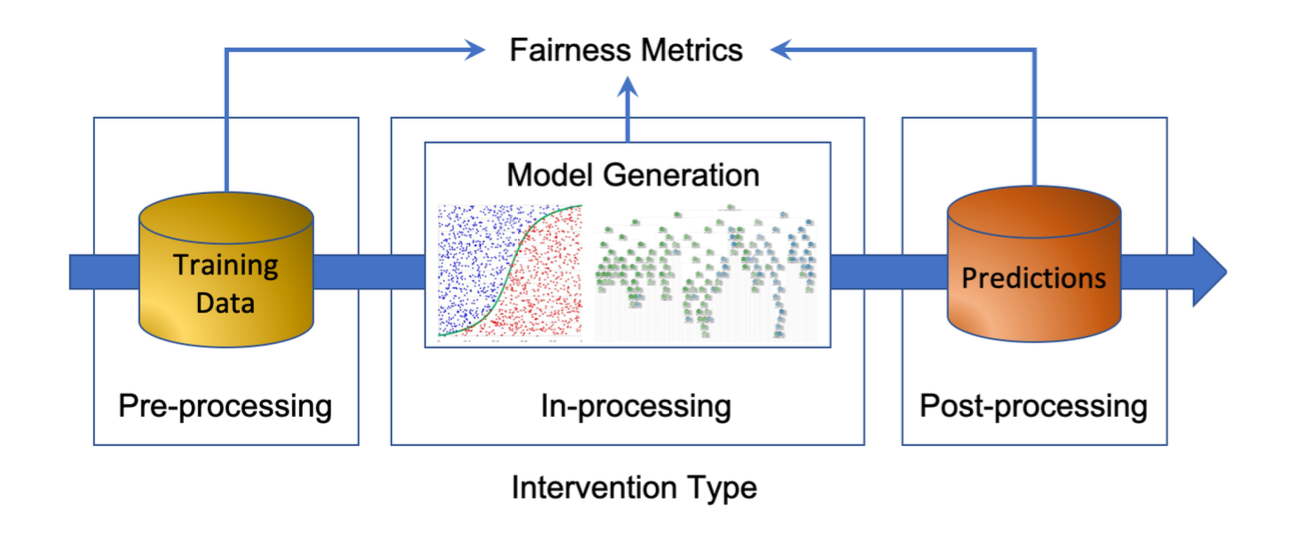
\includegraphics[width=0.6\textwidth]{../figures/fairness_methods.png}
    \caption{Fairness methods can be applied at different stages of the machine learning pipeline \parencite{caton2024}.}
\end{figure}
\section{Sources of bias and the feedback loop}
% insert image
\begin{figure}[h]
    \centering
    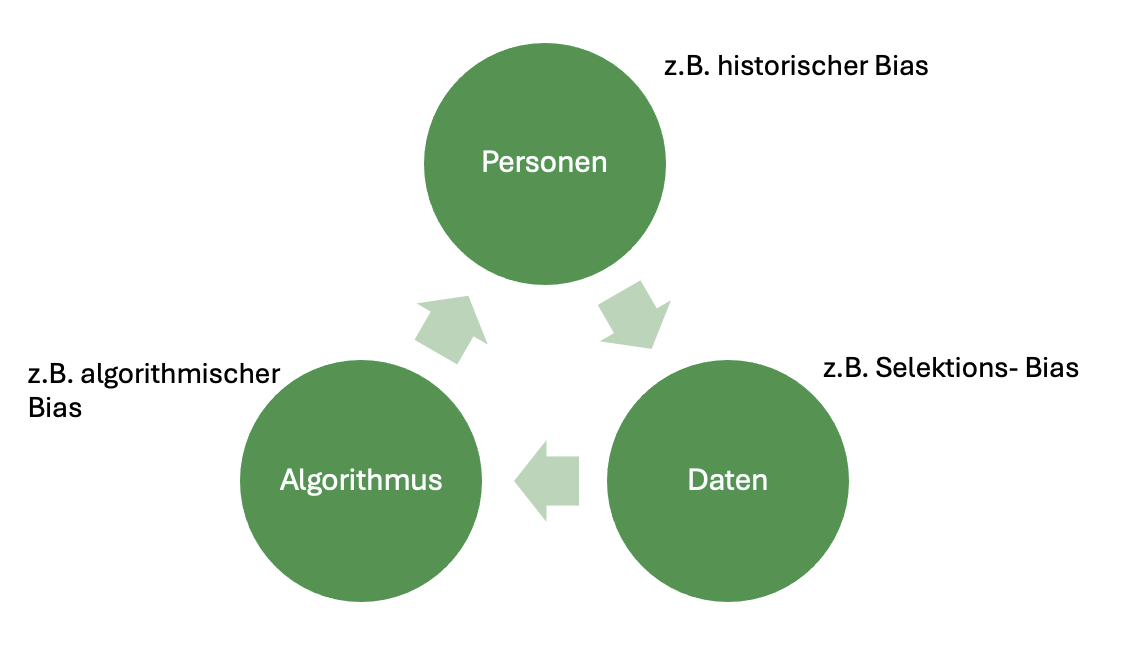
\includegraphics[width=0.6\textwidth]{../figures/bias_loop.png}
    \caption{Bias can come into the process at any stage of the data, algorithm, and user feedback loop \parencite{mehrabi2022}.}
\end{figure} 

% References
\renewcommand{\bibfont}{\scriptsize}  % Set bibliography font size globally
\printbibliography


\end{document}